\chapter{Presentation of the basis of this work} \label{Chapter3}
This thesis is based on the paper \cite{Startingpoint} by Botarelli.
There, a quantum router on the topology of a graph with six nodes
(see \autoref{fig:botarellis_topo}) was analyzed which will be explained in this chapter.
In the next chapter, this will be adapted to an atomic system.

\begin{figure}[!ht]
    \centering
    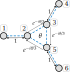
\includegraphics[width=0.5\textwidth]{Botarellis_Topo}
%    \decoRule
    \caption{The minimal graph of the quantum router in \cite{Startingpoint}.
    The circles correspond to nodes and the arrows indicate edges, the interaction between the nodes.
    Small arrows point from each node to their label (a number from 1 to 6).
    The edges with a phase point only in one direction, because the interaction is not symmetric.
    The inner loop carries weights that add up to a phase $\theta$.
    Eq. \eqref{eq:Bot_Hamilton} describes the graph intirely.}
    \label{fig:botarellis_topo}
\end{figure}

\noindent
Graphs are mathematical structures used to model pairwise relations between $N$ nodes.
In this context, nodes represent quantum objects and edges represent interactions between them.
On such a system, classical information is defined as an excitation of one of the nodes.
The node-basis trivially corresponds to the Euclidean basis
\begin{equation}
\vert i\rangle\equiv(0,\dots,\underbrace{1}_{i},\dots,0)^T\text{, for } \alpha = 1, ..., N.
\end{equation}

\noindent
indicating a classical excitation of the $i$-th node.
The quantum mechanical extension of information would be the superposition of classical excitations of nodes.
A Laplacian matrix $ L $ encodes the connectivity of a classical graph.
% Key objects are the adjacency matrix, , and degree matrix
Bottarelli's work extends the Laplacian matrix to allow for complex entries, resulting in a Hermitian Hamiltonian $ H $.
The interactions between two nodes is the complex conjugate of the reverse interaction.
The topology that was analyzed is depicted in \autoref{fig:botarellis_topo} and can be described by the $ 6 \times 6 $ matrix\footnote{The labels of the nodes 4 and 5 were switched in this definition,
    to be consistent with the definition of the system used later in this thesis.
    Such a relabeling has no effect on the physical properties.}

\begin{equation} \label{eq:Bot_Hamilton}
H
=
\begin{pmatrix}
0 & 1 & 0 & 0 & 0 & 0 \\
1 & \gamma & e^{-i \theta / 3} & 0 & e^{i \theta / 3} & 0 \\
0 & e^{i \theta / 3} & \gamma & 1 & e^{-i \theta / 3} & 0 \\
0 & 0 & 1 & 0 & 0 & 0 \\
0 & e^{-i \theta / 3} & e^{i \theta / 3} & 0 & \gamma & 1 \\
0 & 0 & 0 & 0 & 1 & 0
\end{pmatrix},
\end{equation}

\noindent
where specific edges carry a phase given by $\theta$.
The nodes of the inner triangle are connected to themselves, by a factor $ \gamma $.
The identification of the Hamiltonian $ H $
representing the interaction allows the use of quantum mechanical time evolution
to evolve an initial excitation
($\vert \psi (t = 0) \rangle = \sum_{\alpha = 1}^{6} c_\alpha(t = 0) \vert \alpha \rangle $) on the system.
The evolution breaks the time-reversal symmetry, one says it is chiral, because of the phase in the Hamiltonian.
This system-defining parameter is obtained when going along the loop in the graph \autoref{fig:botarellis_topo}.
It is the only quantum part of this analysis, enabling chirality and thus directional routing of information \cite{Ann_Springer, Shu2024}.
The result of Botarelli was that a phase-dependant directional transport of the classical state $\vert \psi_0 \rangle = \vert 1 \rangle $ is possible and robust.
This is shown in \autoref{fig:The_Basis_evolution}.
After a time $T$ a high probability can be achieved to route the initial state into one of the nodes
$ \vert 5 \rangle / \vert 6 \rangle$ while a low probability of being routed into the other nodes $\vert 6 \rangle / \vert 5 \rangle $ is guaranteed.

\begin{figure}[!ht]
    \centering
    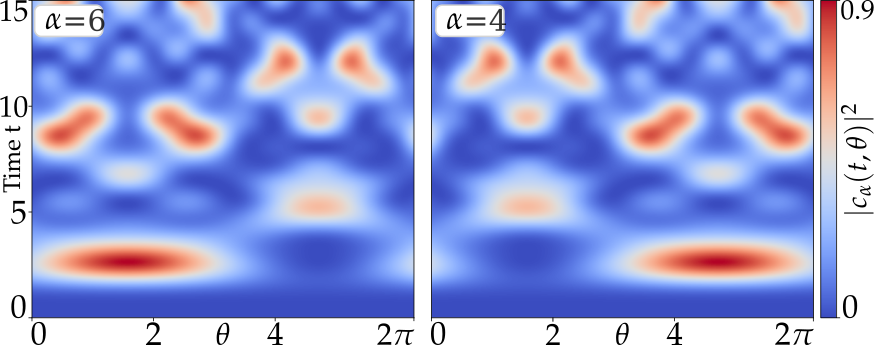
\includegraphics[width=0.8\textwidth]{The_Basis_evolution}
%    \decoRule
    \caption{The probabilities $ |c_\alpha(t) |^2 $ with $ c_1(0) = 1 $  plottet against time $t$ and the total phase $\theta$ of the loop in \autoref{fig:botarellis_topo}.}
    \label{fig:The_Basis_evolution}
\end{figure}

\noindent
The phase in the triangle is not necessary to be equally distributed along the three connections.
The evolution is only dependent on the total phase $ \theta $.
However, a symmetrical allocation makes analytical calculations manageable.

%\begin{figure}[h!]
%    \centering
%    \begin{minipage}{0.5\textwidth}
%        \begin{equation} \label{eq:Bot_Hamilton}
%            H\footnotemark
%            =
%            \begin{pmatrix}
%                0 & 1 & 0 & 0 & 0 & 0 \\
%                1 & \gamma & e^{-i \theta / 3} & 0 & e^{i \theta / 3} & 0 \\
%                0 & e^{i \theta / 3} & \gamma & 1 & e^{-i \theta / 3} & 0 \\
%                0 & 0 & 1 & 0 & 0 & 0 \\
%                0 & e^{-i \theta / 3} & e^{i \theta / 3} & 0 & \gamma & 1 \\
%                0 & 0 & 0 & 0 & 1 & 0
%            \end{pmatrix}.
%        \end{equation}
%    \end{minipage}%
%    \hfill
%    \begin{minipage}{0.45\textwidth}
%        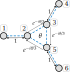
\includegraphics[width=0.8 \textwidth]{Botarellis_Topo}
%    \end{minipage}
%    \caption{The minimal graph structure used by Botarelli. The inner loop carries edge-weights of gamma. Also along the loop a phase $\theta$.}
%    \label{fig:Equation_and_Graphic}
%    \footnotetext{The indices 4 and 5 were switched in this definition to be consistent with the definition of the system used in this paper. Such a relabeling has no effect on the physical properties.}
%\end{figure}